\documentclass[../main.tex]{subfiles}

\begin{document}

\subsection{Vad är en algoritm?}
En algoritm är en uppsättning instruktioner för hur man, steg för steg, löser en matematisk eller logisk uppgift.\\
Vid programmering, skrivs algoritmer för att instruera datorn till att utföra en viss uppgift.\\
\\
Generellt sett, finns algoritmer överallt i vardagen.
Att följa ett recept vid matlagning. Metoder som används vid addition och division när man räknar. Att vika ett par byxor eller en tröja. Din morgonrutin. Kan alla anses vara algoritmer.\\
\\
\textbf{\textit{\say{Algoritmer kan uttryckas på många olika sätt.
Ett vanligt sätt är att algoritmen anges i psuedokod.
Man kan också använda strukturdiagram.}}}\\
\\
\textbf{Förklara skillnaden mellan psuedokod och strukturdiagram}\\
\\
Innan en algoritm designas är det viktigt att först förstå vad problemet är.
\subsubsection{Psuedokod}
Programmerare använder sig utav programspråk som följer en viss syntax, för att få sina program att exekveras ordentligt.\\
Psuedokod är däremot inget programmeringspråk, utan en enklare metod till att beskriva instruktioner utan att behöva trassla med något specifikt syntax. Det finns ingen strikt uppsättning av standardiserad notation för psuedokod. Vilket underlättar att forma instruktioner som sedan kan bildas till programtext samt ger överblick av problemet.

\newpage

\subsubsection{Strukturdiagram}
\begin{wrapfigure}{r}{0.3\textwidth}
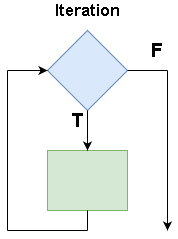
\includegraphics[width=3cm, height=4cm]{sec1/Figs/iteration.png}
\end{wrapfigure}
I strukturdiagram används figurer för illustrativ beskrivning av olika steg i program. Exempel, en diamant-figur symboliserar val i ett program.\\
\\
Ett strukturdiagram är utmärkt till att överblicka program, men blir otympliga vid mer detaljerade nivåer av programmen.



\end{document}